\chapter[Algoritmos de búsqueda]{Algoritmos de búsqueda}

\section{El problema de la búsqueda}

Presentamos ahora uno de los problemas más clásicos de la computación, {\it el
problema de la búsqueda}, que se puede enunciar de la siguiente manera:

{\bf Problema: } Dada una lista $xs$ y un valor $x$ devolver el índice de $x$
en $xs$ si $x$ está en $xs$, y $-1$ si $x$ no está en $xs$.

Alicia Hacker afirma que este problema tiene una solución muy sencilla en
Python: se puede usar directamente la poderosa función \lstinline+index()+ de
lista.

Probamos esa solución para ver qué pasa:

\begin{codigo-python-sn}
>>> [1, 3, 5, 7].index(5)
2
>>> [1, 3, 5, 7].index(20)
Traceback (most recent call last):
  File "<stdin>", line 1, in <module>
ValueError: list.index(x): x not in list
\end{codigo-python-sn}

Vemos que usar la función \lstinline+index()+ resuelve nuestro problema si el
valor buscado está en la lista, pero si el valor no está no sólo no devuelve
un $-1$, sino que se produce un error.

El problema es que para poder aplicar la función \lstinline+index()+ debemos
estar seguros de que el valor está en la lista, y para averiguar eso Python
nos provee del operador \lstinline+in+:

\begin{codigo-python-sn}
>>> 5 in [1, 3, 5, 7]
True
>>> 20 in [1, 3, 5, 7]
False
\end{codigo-python-sn}

O sea que si llamamos a la función \lstinline+index()+ sólo cuando el
resultado de \lstinline+in+ es verdadero, y devolvemos $-1$ cuando el
resultado de \lstinline+in+ es falso, estaremos resolviendo el problema
planteado usando sólo funciones provistas por Python. La solución se plantea a
continuación:

\begin{codigo-python-sn}
def busqueda_con_index(xs, x):
    """Busca un elemento x en una lista xs.

    Si x está en xs devuelve el índice,
    de lo contrario devuelve -1.
    """
    if x in xs:
        return xs.index(x)
    else:
        return -1
\end{codigo-python-sn}

Probamos la función \verb+busqueda_con_index()+:

\begin{codigo-python-sn}
>>> busqueda_con_index([1, 4, 54, 3, 0, -1], 1)
0
>>> busqueda_con_index([1, 4, 54, 3, 0, -1], -1)
5
>>> busqueda_con_index([1, 4, 54, 3, 0, -1], 3)
3
>>> busqueda_con_index([1, 4, 54, 3, 0, -1], 44)
-1
>>> busqueda_con_index([], 0)
-1
\end{codigo-python-sn}

\subsection*{¿Cuántas comparaciones hace este programa?}

Es decir, ¿cuánto esfuerzo computacional requiere
este programa? ¿Cuántas veces compara el valor que buscamos con los datos de
la lista? No lo sabemos porque no sabemos cómo están implementadas las
operaciones \lstinline+in+ e \lstinline+index()+. La pregunta queda planteada
por ahora pero daremos un método para averiguarlo más adelante en esta unidad.


\section{Cómo programar la búsqueda lineal a mano}

Nos interesa ver qué sucede si programamos la búsqueda usando operaciones más
elementales, y no las grandes primitivas \lstinline+in+ e \lstinline+index()+.
Esto nos permitirá estudiar una solución que puede portarse a otros lenguajes
que no tienen instrucciones tan poderosas.

Supongamos entonces que en nuestra versión de Python no existen ni \lstinline+in+
ni \lstinline+index()+. Podemos en cambio acceder a cada uno de los elementos
de la lista a través de una construcción \lstinline+for+, y también, por
supuesto, podemos acceder a un elemento de la lista mediante un índice.

\section{Búsqueda lineal}

Diseñamos una solución: Podemos comparar uno a uno los elementos de la
lista con el valor de \lstinline!x!, y retornar el valor de la posición
donde lo encontramos en caso de encontrarlo.

Si llegamos al final de la lista sin haber salido antes de la función es
porque el valor de \lstinline!x! no está en la lista, y en ese caso
retornamos $-1$.

En esta solución necesitamos una variable \lstinline!i! que cuente en cada
momento en qué posición de la lista estamos parados. Esta variable se
inicializa en $0$ antes de entrar en el ciclo y se incrementa en $1$ en
cada paso.

El programa nos queda entonces como se muestra a continuación:

\begin{codigo-python}
def busqueda_lineal(lista, x):
    """Si x está en lista devuelve su posición en lista, de lo
    contrario devuelve -1.
    """

    i = 0
    for z in lista:
        if z == x:
            return i
        i += 1
    return -1
\end{codigo-python}

Y ahora lo probamos:

\begin{codigo-python-sn}
>>> busqueda_lineal([1, 4, 54, 3, 0, -1], 44)
-1
>>> busqueda_lineal([1, 4, 54, 3, 0, -1], 3)
3
>>> busqueda_lineal([1, 4, 54, 3, 0, -1], 0)
4
>>> busqueda_lineal([], 42)
-1
\end{codigo-python-sn}

\subsection*{¿Cuántas comparaciones hace este programa?}

Volvemos a preguntarnos lo mismo que en la sección anterior, pero con el nuevo
programa: ¿cuánto esfuerzo computacional requiere este programa?, ¿cuántas
veces compara el valor que buscamos con los datos de la lista? Ahora podemos
analizar el texto de \lstinline!busqueda_lineal!:

\begin{itemize}
\item La {\bf línea 7} del código es un ciclo que recorre uno a uno los
elementos de la lista, y en el cuerpo de ese ciclo, en la {\bf línea 8} se
compara cada elemento con el valor buscado. En el caso de encontrarlo ({\bf
línea 9}) se devuelve la posición.

\item Si el valor no está en la lista se recorrerá la lista entera, haciendo
una comparación por cada elemento.
\end{itemize}

O sea que si el valor está en la posición $p$ de la lista se hacen $p$
comparaciones, y si el valor no está se hacen tantas comparaciones como
elementos tenga la lista.

Nuestra hipótesis es: {\bf Si la lista crece, la cantidad de comparaciones
para encontrar un valor arbitrario crecerá en forma proporcional al tamaño de
la lista}.

Diremos que este algoritmo tiene un comportamiento {\it proporcional a la
longitud de la lista involucrada}, o que es un algoritmo {\it lineal}.

En la próxima sección veremos cómo probar esta hipótesis.

\section{Buscar sobre una lista ordenada}

Por supuesto que si la lista está ordenada podemos hacer lo mismo que antes,
con algunas modificaciones que den cuenta de la condición de ordenada de la
lista.

\ejercicioc{Modificar la búsqueda lineal para el caso de listas ordenadas.
¿Cuál es nuestra nueva hipótesis sobre comportamiento del algoritmo?}

\section{Búsqueda binaria}

¿Podemos hacer algo mejor? Trataremos de aprovechar el hecho de que la lista
está ordenada y vamos a hacer algo distinto: nuestro espacio de búsqueda se
irá achicando a segmentos cada vez menores de la lista original.
La idea es descartar segmentos de la lista donde el valor seguro que no puede
estar:

\begin{enumerate}
\item Consideramos como segmento inicial de búsqueda a la lista completa.

\item Analizamos el punto medio del segmento (el valor central), si es el valor
buscado, devolvemos el índice del punto medio.

\item Si el valor central es mayor al buscado, podemos descartar el segmento
que está desde el punto medio hacia la a derecha.

\item Si el valor central es menor al buscado, podemos descartar el segmento
que está desde el punto medio hacia la izquierda.

\item Una vez descartado el segmento que no nos interesa, volvemos a analizar
el segmento restante, de la misma forma.

\item Si en algún momento el segmento a analizar tiene longitud 0 o negativa
significa que el valor buscado no se encuentra en la lista.
\end{enumerate}

Para señalar la porción del segmento que se está analizando a cada paso,
utilizaremos dos variables (\lstinline!izq! y \lstinline!der!) que
contienen la posición de inicio y la posición de fin del segmento que se
está considerando. De la misma manera usaremos la varible \lstinline!medio!
para contener la posición del punto medio del segmento.

En la Figura \ref{fig:busqbin} vemos qué pasa cuando se busca
el valor 18 en la lista [1, 3, 5, 7, 9, 11, 13, 15, 17, 19, 21, 23].

\begin{figure}[h!t]
\begin{center}
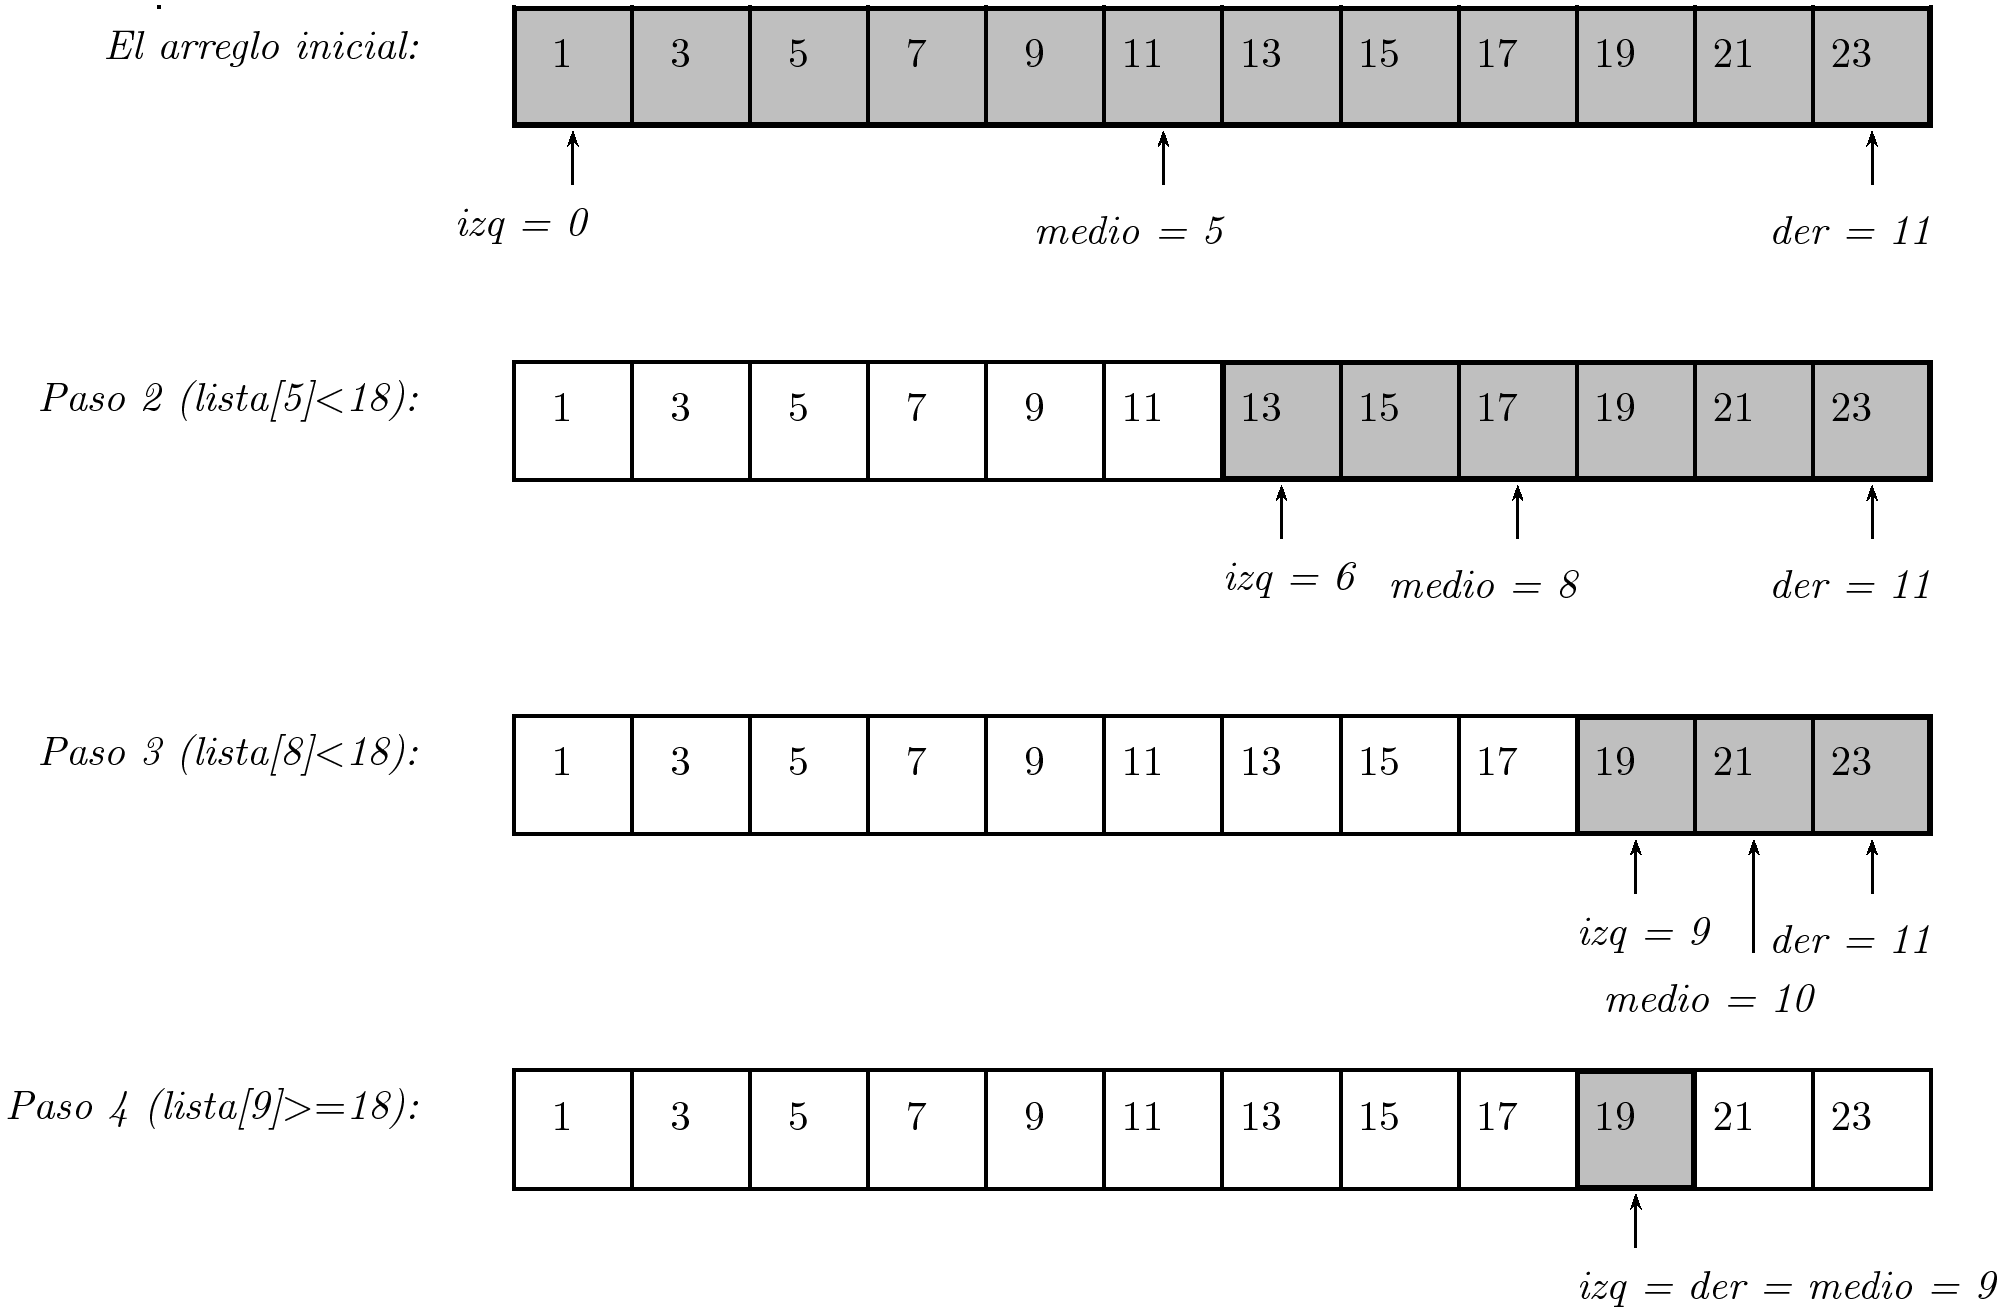
\includegraphics[width=\linewidth]{graficos/uni8-seguimiento}
\end{center}
\caption{Ejemplo de una búsqueda usando el algoritmo de búsqueda binaria.
Como no se encontró al valor buscado, devuelve $-1$.}
\label{fig:busqbin}
\end{figure}

En el Código \ref{busquedabinaria} mostramos una posible implementación de
este algoritmo.

\begin{codigo}{busqueda\_binaria.py}{Función de búsqueda binaria}
\label{busquedabinaria}
\lstinputlisting{src/8_busqueda/busb.py}
\end{codigo}

A continuación varias ejecuciones de prueba:

\begin{codigo-python-sn}
>>> busqueda_binaria([1, 3, 5], 0)
[DEBUG] izq: 0 der: 2 medio: 1
[DEBUG] izq: 0 der: 0 medio: 0
-1
>>> busqueda_binaria([1, 3, 5], 1)
[DEBUG] izq: 0 der: 2 medio: 1
[DEBUG] izq: 0 der: 0 medio: 0
0
>>> busqueda_binaria([1, 3, 5], 2)
[DEBUG] izq: 0 der: 2 medio: 1
[DEBUG] izq: 0 der: 0 medio: 0
-1
>>> busqueda_binaria([1, 3, 5], 3)
[DEBUG] izq: 0 der: 2 medio: 1
1
>>> busqueda_binaria([1, 3, 5], 5)
[DEBUG] izq: 0 der: 2 medio: 1
[DEBUG] izq: 2 der: 2 medio: 2
2
>>> busqueda_binaria([1, 3, 5], 6)
[DEBUG] izq: 0 der: 2 medio: 1
[DEBUG] izq: 2 der: 2 medio: 2
-1
>>> busqueda_binaria([], 0)
-1
>>> busqueda_binaria([1], 1)
[DEBUG] izq: 0 der: 0 medio: 0
0
>>> busqueda_binaria([1], 3)
[DEBUG] izq: 0 der: 0 medio: 0
-1
\end{codigo-python-sn}

\subsection*{¿Cuántas comparaciones hace este programa?}

Para responder esto pensemos en el peor caso, es decir, que se descartaron
varias veces partes del segmento para finalmente llegar a un segmento vacío y
el valor buscado no se encontraba en la lista.

En cada paso el segmento se divide por la mitad y se desecha una de esas
mitades, y en cada paso se hace una comparación con el valor buscado. Por lo
tanto, la cantidad de comparaciones que hacen con el valor buscado es
aproximadamente igual a la cantidad de pasos necesarios para llegar a un
segmento de tamaño 1.
Veamos el caso más sencillo para razonar, y supongamos que la longitud de la
lista es una potencia de 2, es decir \lstinline+len(lista)+$= 2^k$:

\begin{itemize}
\item Luego del primer paso, el segmento a tratar es de tamaño $2^k$.
\item Luego del segundo paso, el segmento a tratar es de tamaño $2^{k-1}$.
\item Luego del tercer paso, el segmento a tratar es de tamaño $2^{k-2}$.

$\ldots$

\item Luego del paso $k$, el segmento a tratar es de tamaño $2^{k-k}=1$.
\end{itemize}

Por lo tanto este programa hace aproximadamente $k$ comparaciones con el valor
buscado cuando \lstinline+len(lista)+$= 2^k$.
Pero si despejamos $k$ de la ecuación anterior, podemos ver que este programa
realiza aproximadamente $\log_2$(\lstinline+len(lista)+) comparaciones.

Cuando \lstinline+len(lista)+ no es una potencia de 2 el razonamiento es menos
prolijo, pero también vale que este programa realiza aproximadamente
$\log_2$(\lstinline+len(lista)+) comparaciones.

\begin{observacion}
Vemos entonces que si \lstinline!lista! es una lista ordenada, la búsqueda binaria es
{\bf muchísimo} más eficiente que la búsqueda lineal.
\end{observacion}

Veamos un ejemplo para entender cuánto más eficiente es la búsqueda binaria.
Supongamos que tenemos una lista de un millón de elementos.

\begin{itemize}
\item El algoritmo de búsqueda lineal hará una cantidad de operaciones proporcional
a un millón; es decir que en el peor caso hará 1.000.000 de comparaciones, y en
un caso promedio, 500.000 comparaciones.
\item El algoritmo de búsqueda binaria hará como máximo $\log_2(1\,000\,000)$
comparaciones, o sea ¡no más que 20 comparaciones!.
\end{itemize}

\section{Resumen}

\begin{itemize}

\item La {\bf búsqueda} de un elemento en una secuencia es un
algoritmo básico pero importante. El problema que intenta resolver puede
plantearse de la siguiente manera: Dada una secuencia de valores y un
valor, devolver el índice del valor en la secuencia, si se encuentra, de no
encontrarse el valor en la secuencia señalizarlo apropiadamente.

\item Una de las formas de resolver el problema es mediante la {\bf
búsqueda lineal}, que consiste en ir revisando uno a uno los elementos de
la secuencia y comparándolos con el elemento a buscar.  Este algoritmo no
requiere que la secuencia se encuentre ordenada.

\item Cuando la secuencia sobre la que se quiere buscar está ordenada, se
puede utilizar el algoritmo de {\bf búsqueda binaria}.  Al estar ordenada
la secuencia, se puede desacartar en cada paso la mitad de los elementos,
quedando entonces con una eficiencia algorítmica relativa al
$log($\lstinline!len(secuencia)!$)$. Este algoritmo sólo tiene sentido
utilizarlo sobre una secuencia ordenada.

\item El análisis del comportamiento de un algoritmo puede ser muy engañoso
si se tiene en cuenta el mejor caso, por eso suele ser mucho más
ilustrativo tener en cuenta el {\bf peor caso}.  En algunos casos
particulares podrá ser útil tener en cuenta, además, el {\bf caso
promedio}.
\end{itemize}


\newpage
\section{Ejercicios}

\extractionlabel{guia}
\begin{ejercicio}
Escribir una función que reciba una lista desordenada y un elemento, que:
\begin{partes}
\item Busque todos los elementos coincidan con el pasado por parámetro y
devuelva la cantidad de coincidencias encontradas.
\item Busque la primera coincidencia del elemento en la lista y devuelva su
posición.
\item Utilizando la función anterior, busque todos los elementos que coincidan
con el pasado por parámetro y devuelva una lista con las posiciones.
\end{partes}
\end{ejercicio}


\extractionlabel{guia}
\begin{ejercicio}
Escribir una función que reciba una lista de números no ordenada, que:
\begin{partes}
\item Devuelva el valor máximo.
\item Devuelva una tupla que incluya el valor máximo y su posición.
\item ¿Qué sucede si los elementos son cadenas de caracteres?
\end{partes}
{\bf Nota:} no utilizar \verb!lista.sort()!
\end{ejercicio}


\extractionlabel{guia}
\begin{ejercicio}
{\bf Agenda simplificada} \\
Escribir una función que reciba una cadena a buscar y una lista de tuplas
(nombre\_completo, telefono), y busque dentro de la lista, todas las
entradas que contengan en el nombre completo la cadena recibida (puede
ser el nombre, el apellido o sólo una parte de cualquiera de ellos).
Debe devolver una lista con todas las tuplas encontradas.
\end{ejercicio}


\extractionlabel{guia}
\begin{ejercicio}
{\bf Sistema de facturación simplificado} \\
Se cuenta con una lista ordenada de productos, en la que uno consiste en
una tupla de (identificador, descripción, precio), y una lista de los
productos a facturar, en la que cada uno consiste en una tupla de
(identificador, cantidad). \\
Se desea generar una factura que incluya la cantidad, la descripción, el
precio unitario y el precio total de cada producto comprado, y al final
imprima el total general. \\
Escribir una función que reciba ambas listas e imprima por
pantalla la factura solicitada.
\end{ejercicio}


\extractionlabel{guia}
\begin{ejercicio}
Escribir una función que reciba una lista ordenada y un elemento. Si el
elemento se encuentra en la lista, debe encontrar su posición mediante
búsqueda binaria y devolverlo.  Si no se encuentra, debe agregarlo a la
lista en la posición correcta y devolver esa nueva posición. (No utilizar
\verb!lista.sort()!.)
\end{ejercicio}

